\documentclass[a4paper, 12pt]{article}
% math symbols
\usepackage{amssymb}
\usepackage{amsmath}
\usepackage{mathrsfs}
\usepackage{physsummer}


\usepackage{enumitem}
\usepackage[margin = 2cm]{geometry}

\tolerance = 1000
\emergencystretch = 0.74cm



\pagestyle{empty}
\parindent = 0mm

\usetikzlibrary{hobby}

\begin{document}

\begin{center}
  \Large{\textbf{Городской центр физического образования, 10 класс.}\\
  \textit{Серия 12, 11 декабря 2014.}}
\end{center}

\begin{center}
  \Large \textbf{ Что такое энтропия? }
\end{center}

\Large

\task{ Два одинаковых тела, нагретых до разных температур, приводятся
  в тепловой контакт друг с другом. Температуры тел
  уравниваются. Покажите, что при этом процессе энтропия системы
  увеличивается.  }
% Савченко, 5.9.1

\task{ Найдите приращение энтропии 1 кг льда при его плавлении. }
% Савченко, 5.9.2

\task{ Тепловая машина, рабочее тело которой --- 1 моль идеального
  одноатомного газа, работает по замкнутому циклу, изображённому на
  графике. Найдите приращение энтропии в машине за один цикл. }
\begin{center}
  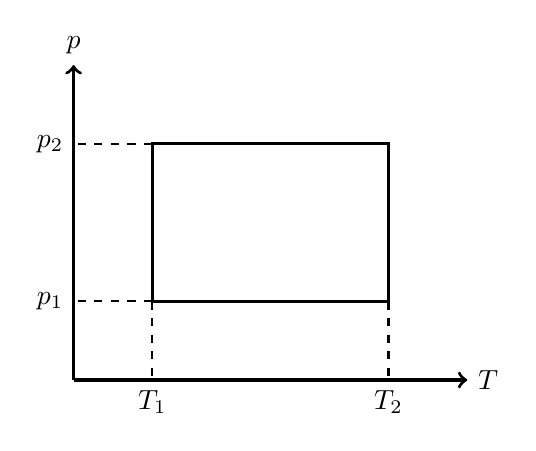
\begin{tikzpicture}
    \draw[very thick,->] (0,0) -- (5,0) node[right] {$T$};
    \draw[very thick,->] (0,0) -- (0,4) node[above] {$p$};
    \draw[very thick] (1,1) rectangle (4,3);
    \draw[thick,dashed] (1,1) -- (0,1) node[left] {$p_1$};
    \draw[thick,dashed] (1,3) -- (0,3) node[left] {$p_2$};
    \draw[thick,dashed] (4,1) -- (4,0) node[below] {$T_2$};
    \draw[thick,dashed] (1,1) -- (1,0) node[below] {$T_1$};
  \end{tikzpicture}
\end{center}


\end{document}


%%% Local Variables: 
%%% mode: latex
%%% TeX-engine:xetex
%%% TeX-PDF-mode: t
%%% End:
